\section{Theoretical background}

A perceptron is a learning algorithm used for binary classification. It is the fundamental computational unit of a neural network and can be viewed 
as a function that maps an input vector \(\mathbf{x}\), whose components are real-valued numbers, to an output \(f(\mathbf{x})\).\footnote{Wikipedia contributors. "Perceptron." Wikipedia, The Free Encyclopedia. Wikipedia, The Free Encyclopedia, 22 Jun. 2026. Web. 18 Jul. 2026.}
To perform binary classification, the perceptron must learn a decision boundary that separates the two classes. In the two-dimensional case considered in this project,
this decision boundary is a straight line (see Fig.~\ref{fig:and-gate}). The perceptron uses a linear model in which each input is multiplied by an associated weight, and a bias term is added:
$ z = w_1x_1 + w_2x_2 + b$

%%%%%%%%%%%%%%%%%%%%%%%%%%%%%%%%%%%%%%%%%%%%% PERCEPTRON %%%%%%%%%%%%%%%%%%%%%%%%%%%%%%%%%%%%%%%%%%%%%%%%%%%%%%%%%%%%%%%%%%%%%%%%%%%%%%
\begin{figure}[ht]
\centering

\begin{minipage}{0.45\textwidth}
    \centering
    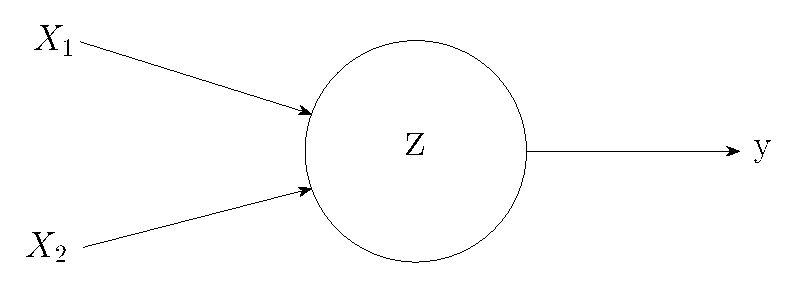
\includegraphics[width=0.9\linewidth]{images/background/perceptron.pdf}
\end{minipage}%
\hfill
\begin{minipage}{0.45\textwidth}
    \centering
    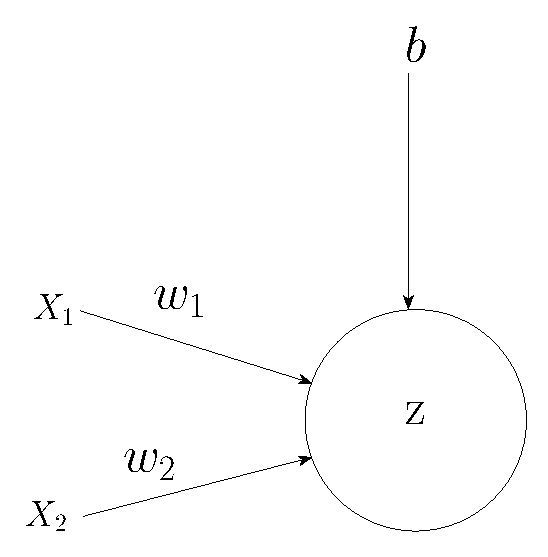
\includegraphics[width=0.6\linewidth]{images/background/background.pdf}
\end{minipage}

\caption{Perceptron figure and linear model with 2 inputs}
\label{fig:perceptron}
\end{figure}

Before being used for prediction, the perceptron is trained on a dataset. The objective of the training process is to determine the optimal values of the weights and the bias so as to minimize the error between the expected output and the prediction produced by the model.
To quantify this error, we use the hinge loss function (described below), which assigns a cost to each prediction according to the expected label. The model parameters are then optimized using the gradient descent algorithm, which iteratively updates the weights and the bias
to minimize the loss function.

Once the perceptron has been trained, it can classify previously unseen data. Given a new input, the linear model computes the value of \(z\),
which indicates on which side of the decision boundary the input lies. Finally, the step activation function converts this value into a binary prediction corresponding to one of the two classes.





%%%%%%%%%%%%%%%%%%%%%%%%%%%%%%%%%%%%%%%%%%%%%% AND GATE %%%%%%%%%%%%%%%%%%%%%%%%%%%%%%%%%%%%%%%%%%%%%%%%%%%%%%%%%%%%%%%%%%%%%%%%%%%%%%%
\begin{figure}[ht]
\centering

\begin{minipage}{0.45\textwidth}
    \centering
    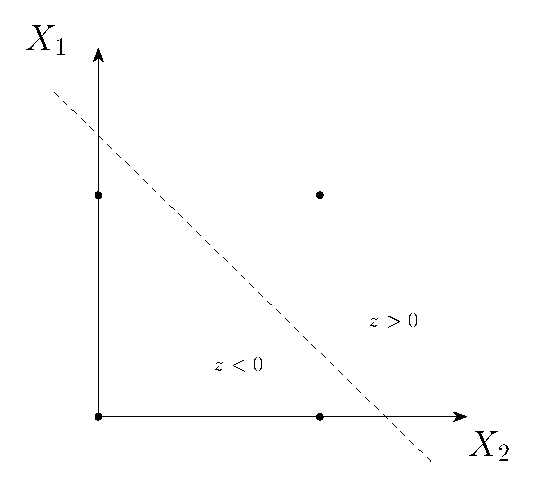
\includegraphics[width=0.9\linewidth]{images/logic_gates/and.pdf}
\end{minipage}%
\hfill
\begin{minipage}{0.45\textwidth}
    \centering
    \LARGE
    \begin{tabular}{c|c|c}
        \textbf{$x_1$} & \textbf{$x_2$} & \textbf{$y$} \\
        \hline
        0      & 0      & 0      \\
        0      & 1      & 0      \\
        1      & 0      & 0      \\
        1      & 1      & 1      \\
    \end{tabular}
\end{minipage}

\caption{Truth table of AND gate and linear separation between the two classes.}
\label{fig:and-gate}
\end{figure}


%%%%%%%%%%%%%%%%%%%%%%%%%%%%%%%%%%%%%%%%%%%%%%% XOR GATE %%%%%%%%%%%%%%%%%%%%%%%%%%%%%%%%%%%%%%%%%%%%%%%%%%%%%%%%%%%%%%%%%%%%%%%%%%%%%%%%%%

\begin{figure}[ht]
\centering

\begin{minipage}{0.45\textwidth}
    \centering
    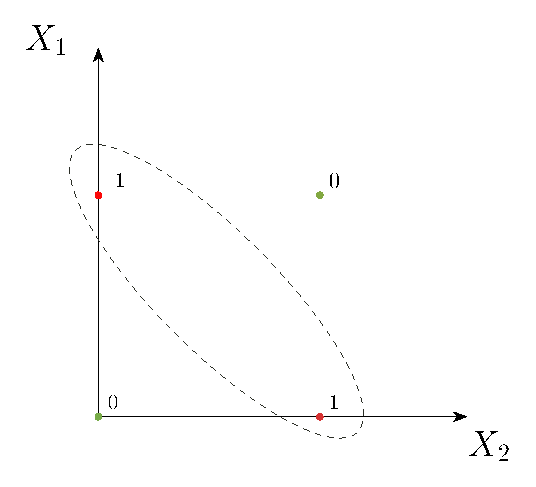
\includegraphics[width=0.9\linewidth]{images/logic_gates/xor.pdf}
\end{minipage}%
\hfill
\begin{minipage}{0.45\textwidth}
    \centering
    \LARGE
    \begin{tabular}{c|c|c}
        \textbf{$x_1$} & \textbf{$x_2$} & \textbf{$y$} \\
        \hline
        0      & 0      & 0      \\
        0      & 1      & 1      \\
        1      & 0      & 1      \\
        1      & 1      & 0      \\
    \end{tabular}
\end{minipage}

\caption{Truth table of XOR gate and non-linear separation between the two classes.}
\label{fig:xor-gate}
\end{figure}

